\documentclass[11pt]{article}
\usepackage[margin=1in]{geometry}
\usepackage{amsmath,amssymb}
\usepackage{graphicx}
\usepackage{hyperref}
\usepackage{booktabs}

% Compile-safe figure slot: replace with \includegraphics when you have the export.
\newcommand{\placeholdfig}[4]{%
  \begin{figure}[htbp]
  \centering
  \fbox{\begin{minipage}{0.9\textwidth}\centering\vspace{#1}
  \textit{\textbf{[PLACEHOLDER --- ParaView / Matplotlib]}}

  #2

  \vspace{0.5em}\footnotesize\textit{Suggested file:} \texttt{#3}
  \vspace{#1}\end{minipage}}
  \caption{#4}
  \end{figure}}

\newcommand{\missing}[1]{\textbf{[TODO:~#1]}}

\title{APMA 4302 Homework 4 \\ Solutions}
\author{Dan}
\date{\today}

\begin{document}
\maketitle

\section*{Problem 1}
In 2D, define
\[
\mathbf{v} = \nabla \times (\psi \hat{\mathbf{k}})
= \left(\frac{\partial \psi}{\partial y}, -\frac{\partial \psi}{\partial x}\right),
\qquad
\omega \hat{\mathbf{k}} = \nabla \times \mathbf{v}.
\]
Taking the scalar curl of $\mathbf{v}$ gives
\[
\omega = \frac{\partial v_y}{\partial x} - \frac{\partial v_x}{\partial y}
= -\frac{\partial^2 \psi}{\partial x^2} - \frac{\partial^2 \psi}{\partial y^2}
= -\nabla^2 \psi,
\]
which is Eq. (6):
\[
-\nabla^2 \psi = \omega.
\]

Start from momentum,
\[
-\nabla^2 \mathbf{v} + \abla p = T \hat{\mathbf{j}}.
\]
Take the scalar curl of both sides. Using $\nabla \times \nabla p = 0$ and
\[
\nabla \times (T\hat{\mathbf{j}}) = \frac{\partial T}{\partial x},
\]
we obtain
\[
-\nabla^2 (\nabla \times \mathbf{v}) = \frac{\partial T}{\partial x}
\;\;\Longrightarrow\;\;
-\nabla^2 \omega = \frac{\partial T}{\partial x},
\]
which is Eq. (5).

The temperature equation is already
\[
\frac{\partial T}{\partial t} + \mathbf{v}\cdot \nabla T
= \frac{1}{Ra}\nabla^2 T,
\]
which is Eq. (4). Therefore Eqs.~(1)--(3) are equivalent to Eqs.~(4)--(6) in streamfunction-vorticity form.

\section*{Problem 2}
\subsection*{(a) C code: convergence and run times}
I ran the C code (\texttt{c/biharm.c}) using PETSc build
\[
\texttt{PETSC\_DIR=/Users/dan/Desktop/Columbia/HPC\_4302/petsc},\quad
\texttt{PETSC\_ARCH=apma4302-pkgs-opt}
\]
with the three provided options files. The key solver metrics are:

\begin{center}
\begin{tabular}{lccc}
\hline
Configuration & KSP iterations & Total wall time (s) & \texttt{SNESSolve} time (s) \\
\hline
\texttt{options\_file\_direct} & 1 & 2.219 & 2.1203 \\
\texttt{options\_file\_split\_direct} & 1 & 2.735 & 2.6370 \\
\texttt{options\_file\_split\_mg} & 4 & 0.7512 & 0.66465 \\
\hline
\end{tabular}
\end{center}

Observations:
\begin{itemize}
  \item The fieldsplit+multigrid configuration is fastest by a large margin (about $3\times$ faster than monolithic direct here).
  \item Fieldsplit+direct is slower than monolithic direct in this test, likely due to extra block-solver overhead without enough reduction in work.
  \item The multigrid case needs more Krylov iterations, but each iteration is much cheaper.
\end{itemize}

\subsection*{(b) Firedrake \texttt{biharm.py}: same three solver presets}
Run on the cluster inside \texttt{firedrake-ts} (see \texttt{hw4/RUN.md}); logs under \texttt{hw4/output/logs/}. Fill in from \texttt{q2\_py\_*.log} or stdout (KSP residual lines + \texttt{-log\_view} if you add it).

\begin{center}
\begin{tabular}{lccc}
\toprule
Preset (\texttt{--preset}) & KSP iterations & Wall time (s) & Notes \\
\midrule
\texttt{direct} & \missing{from log} & \missing{from log} & monolithic LU / MUMPS \\
\texttt{split\_direct} & \missing{from log} & \missing{from log} & fieldsplit, LU blocks \\
\texttt{split\_mg} & \missing{from log} & \missing{from log} & fieldsplit, MG blocks \\
\bottomrule
\end{tabular}
\end{center}

Optional: paste L2 errors printed at end of each run (should match manufactured solution).

\subsection*{(c) One solver set: where does runtime differ (C vs Firedrake)?}
Pick one configuration (e.g.\ \texttt{split\_mg} or \texttt{direct}). Compare representative \texttt{-log\_view} sections (e.g.\ \texttt{SNESSolve}, \texttt{KSPSolve}, matrix assembly, PC setup).

\missing{2--3 sentences: dominant cost in C run vs Firedrake run (e.g.\ FE assembly, different DOF count $513^2$ FD vs FE mesh, sparse direct on larger coupled FE system, etc.).}

\placeholdfig{1.8cm}{%
Bar chart or table summarizing \texttt{SNESSolve} / total time for C vs Python for the \emph{same} preset (optional).%
}{figures/hw4\_q2\_runtime\_compare.pdf}{Optional: runtime comparison C vs Firedrake (Problem 2c).}
% When ready, replace the \placeholdfig block above with:
% \begin{figure}...\includegraphics[width=0.75\textwidth]{figures/hw4_q2_runtime_compare.pdf}...\end{figure}

\section*{Problem 3}
We solve the coupled streamfunction--vorticity system with manufactured temperature
\[
T(x,y) = (1-y) + A\cos(\pi x), \qquad A = 0.1,
\]
and source $f = \partial T / \partial x$ in $-\nabla^2 \omega = f$, $-\nabla^2 \psi = \omega$, with homogeneous Dirichlet data on $\omega$ and $\psi$ on $\partial\Omega$, matching the provided driver \texttt{python/biharm\_temperature\_rhs.py}. VTK is written to \texttt{hw4/output/q3/biharm\_T\_rhs.pvd}.

\placeholdfig{2.0cm}{%
\textbf{ParaView:} show \emph{temperature} as the primary field; overlay \emph{streamfunction} contours; superpose \emph{velocity} vectors (or streamlines) from $\mathbf{v} = \nabla\times(\psi\hat{\mathbf{k}})$. Use a single clear panel suitable for the PDF.%
}{figures/hw4\_q3\_T\_psi\_velocity.pdf}{Temperature field with streamfunction contours and velocity (Problem 3).}

\section*{Problem 4}
Time-dependent convection uses \texttt{python/convection.py} (implicit DAE with \texttt{firedrake-ts}, BDF-2, monolithic MUMPS per step unless you change options). Mesh $N\times N$ Q$_1$ cells; boundary data as in the handout; $Nu$ is written to \texttt{nu\_history.csv}.

\subsection*{(a) $Ra = 10^2$, $64\times 64$, $t_{\max} = 10^5$}
\missing{State whether the long-time state is conductive (no convection), with evidence: e.g.\ $|Nu-1|$, snapshot of $T$ near linear profile, decay of kinetic energy if plotted.}

\placeholdfig{1.6cm}{Optional snapshot of $T$ and/or $\psi$ at late time for $Ra=10^2$.}{figures/hw4\_q4\_Ra1e2\_late.pdf}{Optional: late-time fields for $Ra=10^2$ (4a).}

\subsection*{(b) $Ra = 10^4, 10^5, 10^6$}
\begin{center}
\begin{tabular}{lccc}
\toprule
$Ra$ & Final / steady $Nu$ & Notes (convective pattern, run cost) \\
\midrule
$10^4$ & \missing{from \texttt{nu\_history.csv}} & \missing{} \\
$10^5$ & \missing{} & \missing{} \\
$10^6$ & \missing{} & \missing{} \\
\bottomrule
\end{tabular}
\end{center}

\placeholdfig{1.6cm}{$Nu(t)$ curves for the three $Ra$ (import CSV in Matplotlib / Paraview plot).}{figures/hw4\_q4\_Nu\_vs\_t\_Ra\_sweep.pdf}{$Nu$ vs time for $Ra \in \{10^4,10^5,10^6\}$ (4b).}

\subsection*{(c) $Ra = 10^4$: mesh refinement vs Blankenbach}
Blankenbach benchmark~1 reports $Nu \approx 4.884$ for this configuration (cite / quote as in course notes).

\begin{center}
\begin{tabular}{ccccc}
\toprule
$N$ & $Nu$ (your run) & $|Nu - 4.884|$ & Notes \\
\midrule
16 & \missing{} & \missing{} & \\
32 & \missing{} & \missing{} & \\
64 & \missing{} & \missing{} & \\
128 & \missing{} & \missing{} & \\
\bottomrule
\end{tabular}
\end{center}

\missing{Short discussion: mesh convergence toward $4.884$; cost of $N=128$; any discrepancy due to time truncation, timestep, or BC discretization.}

\placeholdfig{1.6cm}{$Nu$ vs $N$ (log scale optional) with horizontal line at $4.884$.}{figures/hw4\_q4\_Nu\_vs\_N\_Ra1e4.pdf}{$Nu$ vs mesh size for $Ra=10^4$ vs Blankenbach (4c).}

\section*{Problem 5 (Extra credit)}
The handout lists three optional themes. Below: what we implemented, how to run it, and what remains for a ``full'' submission.

\begin{enumerate}
  \item \textbf{Full convergence study for $Ra=10^4,10^5,10^6$.}
  We automate a mesh$\times$Rayleigh sweep by repeatedly calling \texttt{python/bonus\_convergence\_sweep.py} (wrapper: \texttt{hw4/scripts/run\_bonus.sh sweep}). Each case runs \texttt{convection.py} (DAE BDF-2) and records the \emph{final} $Nu$ from \texttt{nu\_history.csv} into \texttt{output/bonus\_convergence/summary\_nu\_final.csv}.

  \emph{Important:} use a large enough \texttt{--t-max} per $(Ra,N)$ so $Nu$ is near steady; the default \texttt{5000} is a compromise for cost. Increase for publication-quality numbers.

  \begin{center}
  \begin{tabular}{rrcc}
  \toprule
  $Ra$ & $N$ & $Nu_{\mathrm{final}}$ (sweep) & Notes \\
  \midrule
  $10^4$ & 16 & \missing{paste from \texttt{summary\_nu\_final.csv}} & \\
  $10^4$ & 32 & \missing{} & \\
  $10^4$ & 64 & \missing{} & \\
  $10^4$ & 128 & \missing{} & \\
  $10^5$ & 16 & \missing{} & \\
  \multicolumn{4}{c}{$\vdots$ \textit{(fill remaining rows from CSV)}} \\
  \bottomrule
  \end{tabular}
  \end{center}

  \placeholdfig{1.5cm}{%
  Plot $Nu_{\mathrm{final}}$ vs $N$ for each $Ra$ (three curves) or a heatmap of $(Ra,N)$.%
  }{figures/hw4\_bonus\_Nu\_mesh\_Ra\_heatmap.pdf}{Extra credit (1): $Nu$ mesh / $Ra$ convergence summary.}

  \item \textbf{PETSc C + \texttt{DMDA} + \texttt{TS} with fieldsplit.}
  A faithful port mirrors \texttt{convection.py}: coupled temperature + vorticity + streamfunction on a staggered or collocated grid, nonlinear advection, implicit time stepping, and block preconditioners analogous to \texttt{biharm.c}. This is a substantial separate code path (context structs, \texttt{FormFunctionLocal}, Jacobian, \texttt{TSSetIJacobian}, MG levels per block). \missing{Not implemented here; outline only unless you extend \texttt{hw4/c/} with a new driver and verify against Firedrake on a coarse grid.}

  \item \textbf{Crank--Nicolson in time / FE in space, SNES per step, plain Firedrake + block PCs.}
  We provide \texttt{python/convection\_cn.py}: each time step solves one monolithic SNES for $(T^{n+1},\omega^{n+1},\psi^{n+1})$ with CN on the temperature equation (midpoint in $T$ and $\psi$ for $\mathbf{v}$). Default linear solver is monolithic LU/MUMPS; you may swap in \texttt{fieldsplit} + MG in \texttt{snes\_params} for the bonus wording.

  Run (\texttt{hw4/scripts/run\_bonus.sh cn} or directly \texttt{python3 convection\_cn.py \ldots}) and compare \texttt{nu\_history\_cn.csv} to BDF-2 \texttt{convection.py} at the same $(Ra,N,\Delta t,t_{\max})$.

  \missing{1--2 paragraphs: agreement or drift in $Nu(t)$; CN timestep stability vs cost of nonlinear solves per step.}

  \placeholdfig{1.5cm}{Overlay $Nu(t)$ from \texttt{convection.py} vs \texttt{convection\_cn.py}.}{figures/hw4\_bonus\_Nu\_bdf\_vs\_cn.pdf}{Extra credit (3): BDF-2 (DAE) vs Crank--Nicolson (SNES per step).}
\end{enumerate}

\appendix
\section*{Assignment handout (reference)}
\begin{figure}[h!]
  \centering
  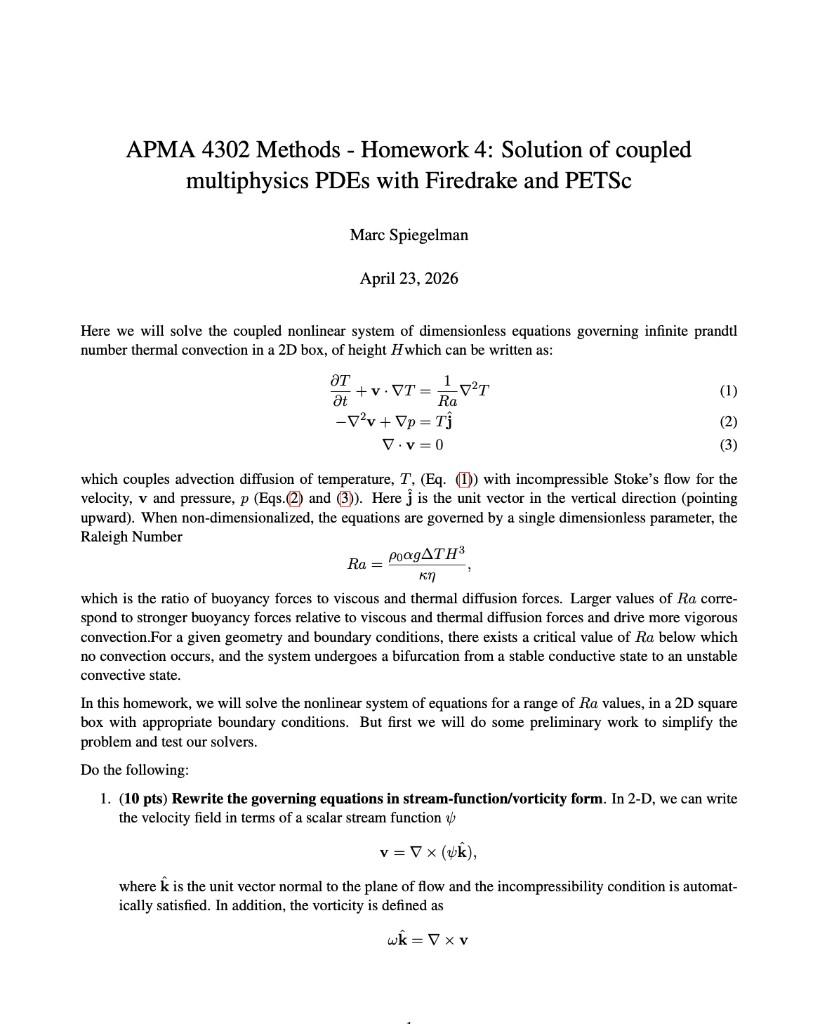
\includegraphics[width=\textwidth]{figures/hw4_1.png}
  \caption{Homework 4 page 1.}
\end{figure}

\begin{figure}[h!]
  \centering
  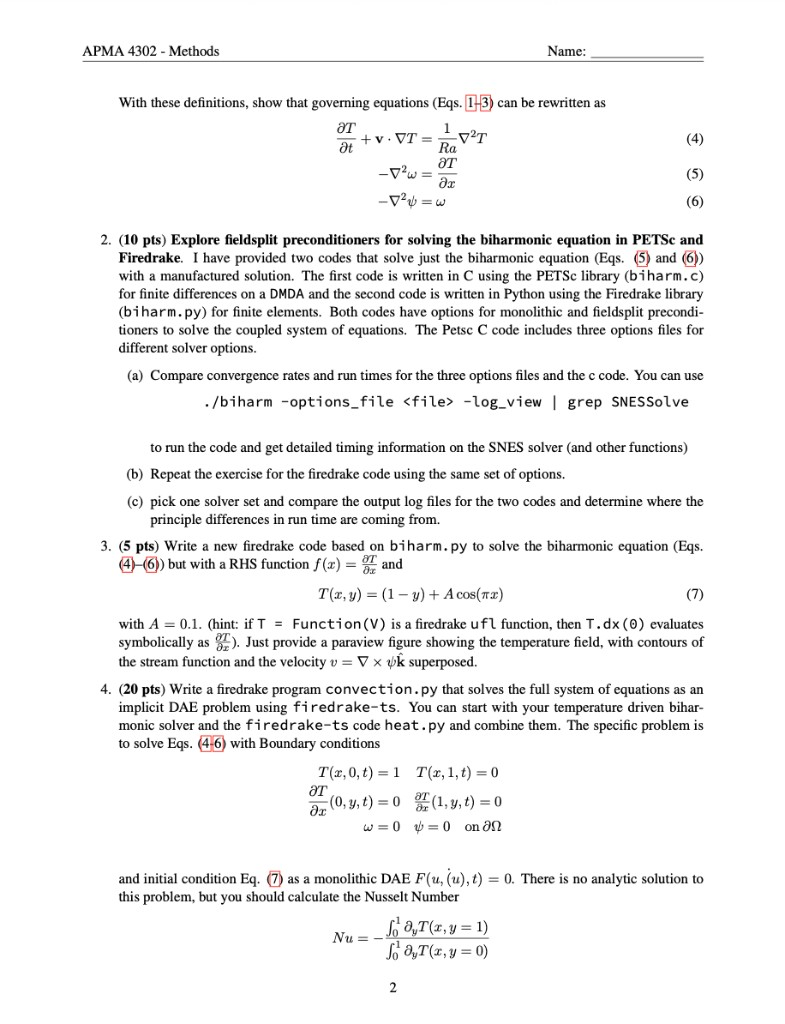
\includegraphics[width=\textwidth]{figures/hw4_2.png}
  \caption{Homework 4 page 2.}
\end{figure}

\begin{figure}[h!]
  \centering
  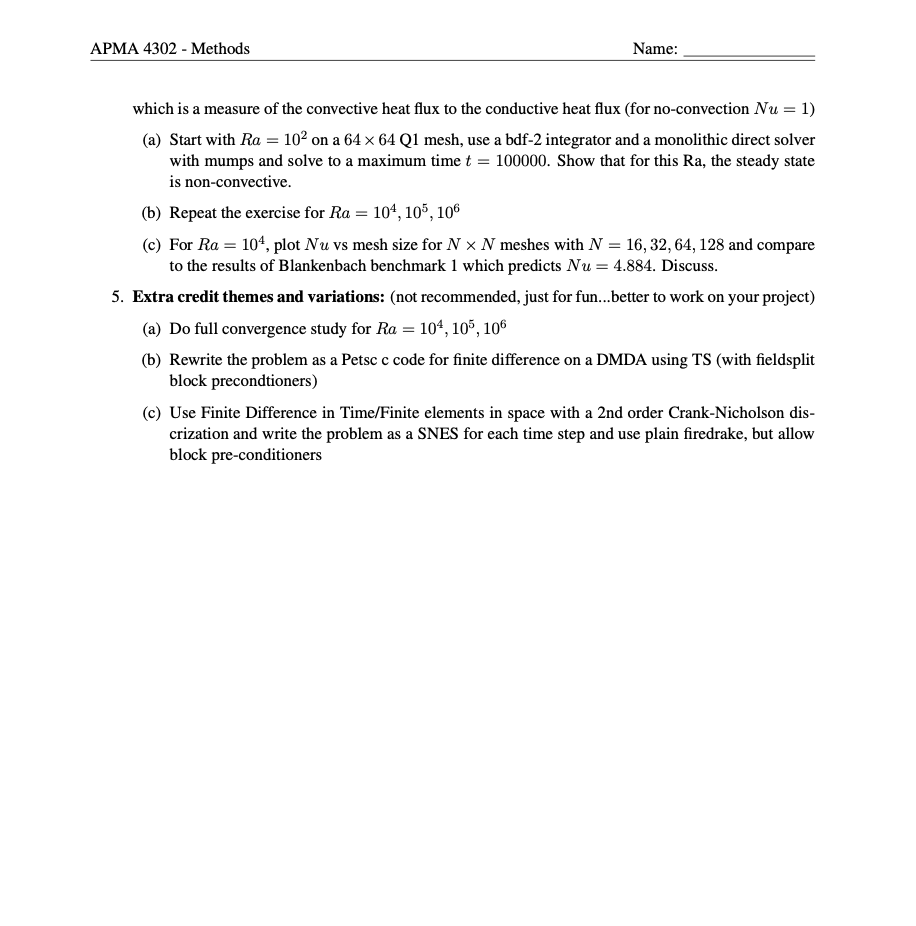
\includegraphics[width=\textwidth]{figures/hw4_3.png}
  \caption{Homework 4 page 3.}
\end{figure}

\end{document}
